\chapter{Performance}
\label{ch:performance} 
	Unless otherwise specified the following tests were performed using two CPUs or two GPUs, with MPI as the interface between multiple threads. The machine specifications are as follows:
\begin{itemize}
	\item CPU: Intel Core i7 930 @ 2.8GHz.
	\item Memory: 12GB (3 x 4GB) DDR3 - 1333MHz ECC Unbuffered Server memory. 
	\item GPUs: 2x EVGA GeForce GTX 470 1280MB, 607 MHz / 1215 MHz, Graphics / Processor Clock. 
	\item Motherboard: ASUS P6T7 WS Cupercomputer Intel x58.
\end{itemize}
%	\section{Test Setup}
%		\subsection{Parameter Space Explored}
%		\subsection{Machine Parameters}
%		\subsection{Memory Bandwidth Comparison}

Typical total\footnote[1]{Total run time includes MPI reduces and various other subroutines that were not ported to the GPU} speedups on this setup are on the order of 40x. A detailed breakdown of the run times per particle per time step and the speedup achieved by the GPU can be seen in table \ref{tab:speedup}. This run was performed on 2 GPUs with 17 million particles per GPU and a grid size of $64^3$.

\noindent \begin{figure}
\begin{center}
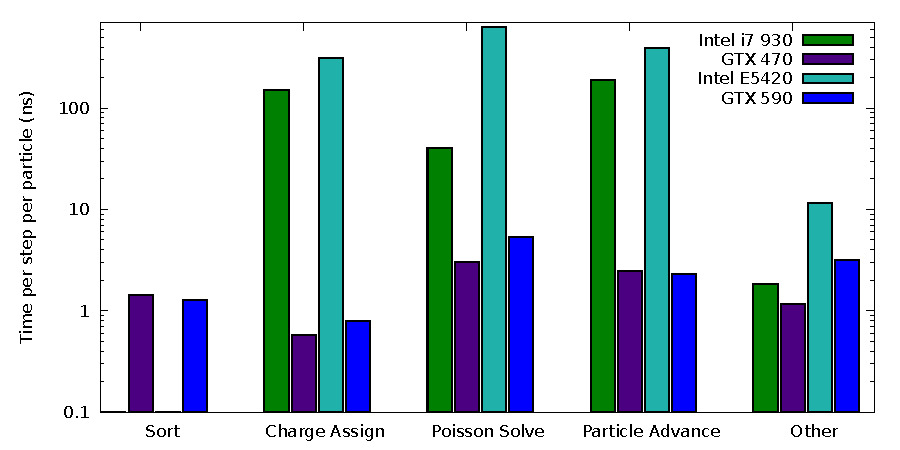
\includegraphics[width=6in]{performance/architecture_compare.pdf}
\end{center}
\caption{CPU and GPU Runtime comparison for a GTX 590 vs an Intel(R) Xeon(R) CPU E5420. Test was performed using 2 MPI threads handling 17 million particles each on a $64^3$ grid.}
\label{tab:speedup2} 
\end{figure} 

\noindent \begin{figure}
\begin{center}
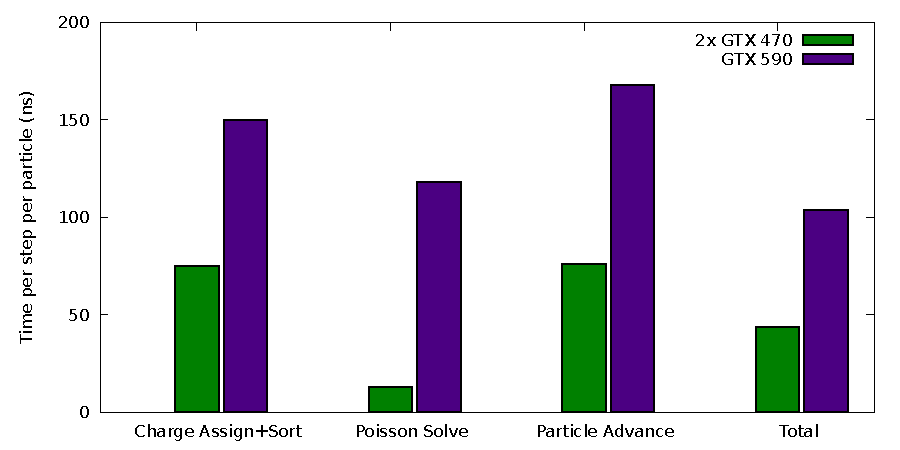
\includegraphics[width=6in]{performance/architecture_speedup_compare.pdf}
\end{center}
\caption{CPU and GPU Runtime comparison for a GTX 590 vs an Intel(R) Xeon(R) CPU E5420. Test was performed using 2 MPI threads handling 17 million particles each on a $64^3$ grid.}
\label{tab:speedup2} 
\end{figure} 



The initial results indicate that a very high speedup was achieved for the charge assign and particle advance routines. It should also be noted that ordering the particle data allows for an incredibly fast charge assign. After accounting for the time that it takes to sort the particle list, the speedup is a more modest 75x. In other codes the primary concern has been how to quickly and efficiently keep the particle list sorted. The results in table \ref{tab:speedup} indicate, that with the latest thrust sort, that speeding up the particle list sort is no longer a major issue. The sort step could be improved by taking into account problem specific properties of a given pic code, but considering the ease of implementation and generality of the thrust sort, it is unlikely that developing an optimized problem-specific sorting routine would really be worth it. 

We also compared the performance between single and double gpu cards, as well as performance on different CPU architectures. Table \ref{tab:speedup2} shows the run times for the CPU and GPU on a machine with 2x  Intel(R) Xeon(R) CPU E5420 @ 2.50GHz and 1x NVIDIA GeForce GTX 590. The GTX 590 is a double GPU card with 2 x 512 processing cores clocked at 630 MHz, and 2x 1.5 GB ram. 

	
	\section{Particle list size scan}
The following tests were performed to explore the dependence of sceptic3Dgpu's runtime on the total number of particles in the simulation for two standard grid sizes. Figure \ref{fig:nptclsize_scan128x64x64} was performed on a 128x64x64 grid, and figure \ref{fig:nptclsize_scan64x32x32} was performed on a 64x32x32 grid. Since the run times for the GPU and the CPU vary by such a large degree, a comparison between the two architectures is represented by the speedup factor, $\tau_{\mathrm{cpu}}/\tau_{\mathrm{gpu}}$. The speedup factor as a function of the total number of particles is shown in \ref{fig:nptclsize_scan_speedup}.

\begin{figure}
\begin{center}
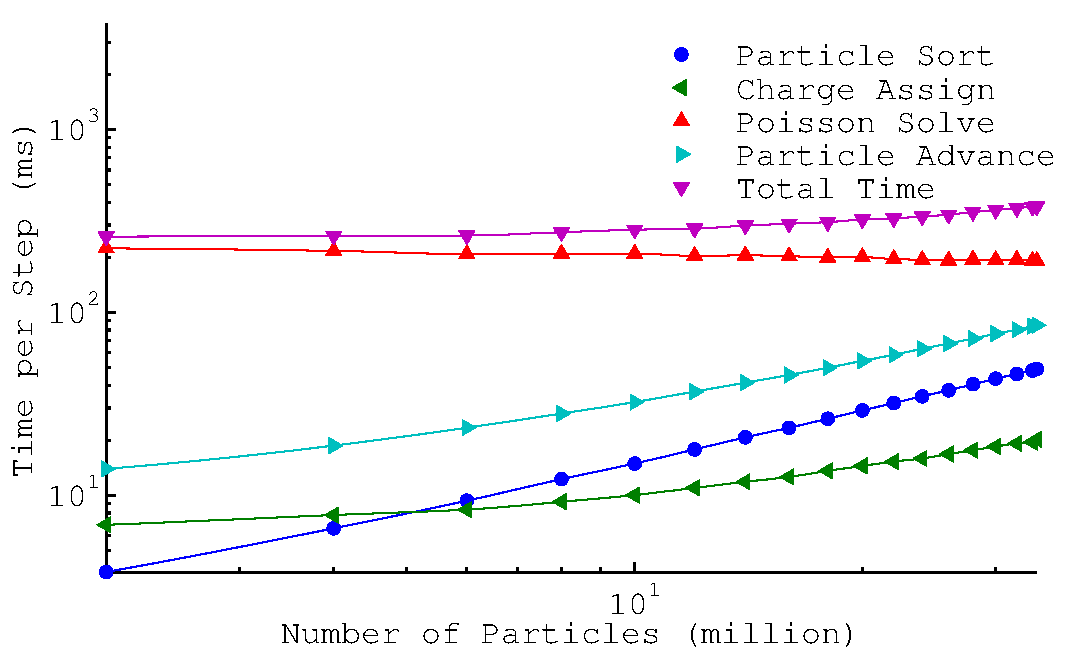
\includegraphics[width=6in]{performance/nptclsize_scan128x64x64ons8bins.pdf}
\end{center}
\caption{Number of Particles Scan on a 128x64x64 grid}
\label{fig:nptclsize_scan128x64x64}
\end{figure}

\begin{figure}
\begin{center}
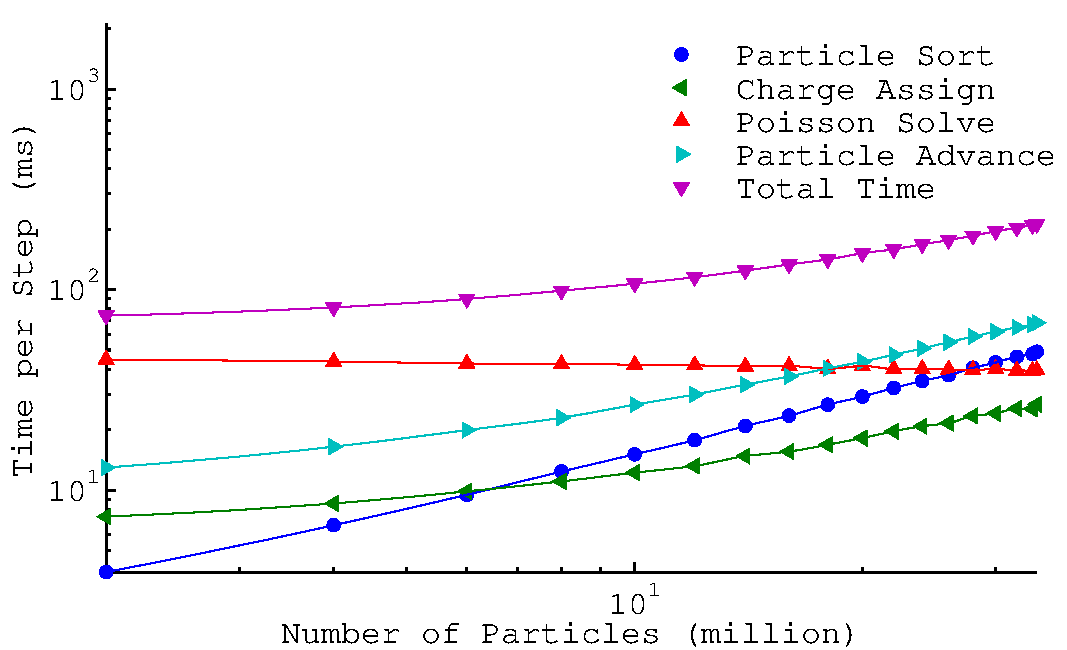
\includegraphics[width=6in]{performance/nptclsize_scan64x32x32ons8bins.pdf}
\end{center}
\caption{Number of Particles Scan on a 64x32x32 grid}
\label{fig:nptclsize_scan64x32x32}
\end{figure}

\begin{figure}
\begin{center}
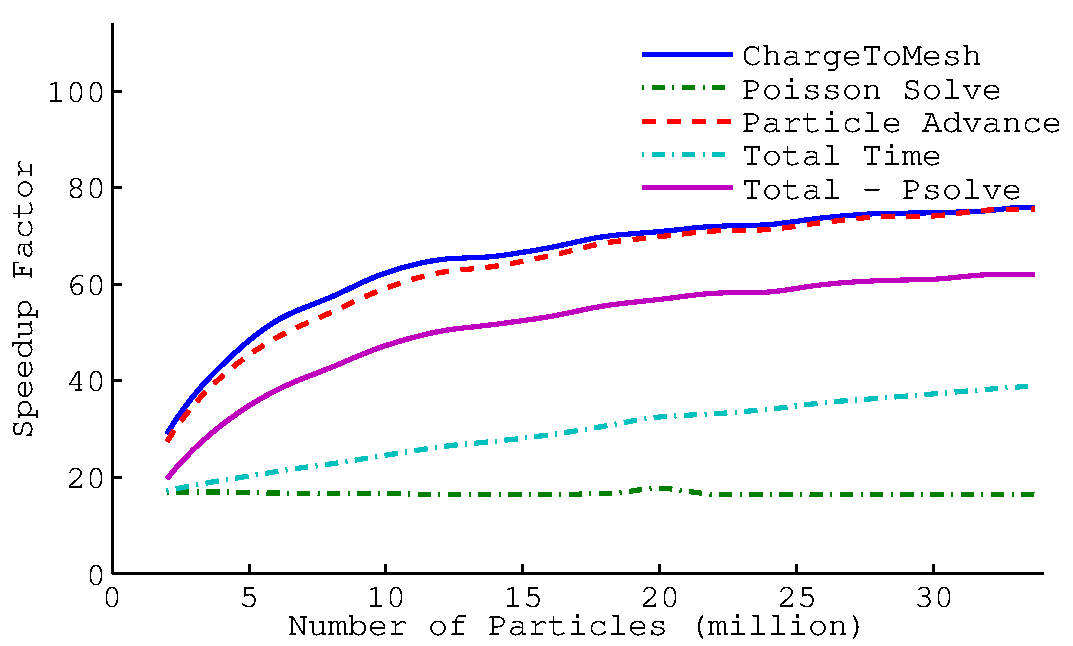
\includegraphics[width=6in]{performance/nptclspeedup_scan128x64x64ons8bins.pdf}
\end{center}
\caption{Speedup factor Number of Particles Scan on a 128x64x64 grid}
\label{fig:nptclsize_scan_speedup}
\end{figure}

In the case of the 128x64x64 grid the poisson solve is by far the most expensive computation for all ranges of particles. For a smaller grid, 64x32x32, the poisson solve dominates for fewer than 15 million particles, but drops below the particle advance and particle sort for more than 15 million particles. Perhaps the most interesting behavior is best observed in the speedup factor, figure \ref{fig:nptclsize_scan_speedup}, which shows a very steep rise in the speedup factor below 10 million particles. This behavior indicates that anything fewer than 10 million particles will not saturate the gpu. This behavior can also be seen in the figures \ref{fig:nptclsize_scan128x64x64} and \ref{fig:nptclsize_scan64x32x32} by the fact that the particle advance, charge assign, and total time converge to linear behavior at large numbers of particles. 

A second interesting characteristic is the fact that the speedup factor curves do not fully flatten out between 10 million particles and 30 million particles. This is due in part to some small cpu costs within these routines, namely host-device transfers of data that does not scale with the number of particles. For the GTX 470 with 1280 MB of memory 17 million particles is about the limit for a single gpu. Looking at figure \ref{fig:nptclsize_scan_speedup} it is not unreasonable to conclude that with an even larger performance boost can be attained simply by increasing the amount of available device memory.

	
\section{Grid Size scan}
So far the results indicate that the GPU is very good at moving the particles and writing the density array. In fact the GPU is so good at this that it is wasteful to not run as many particles on the gpu as physically possible. This brings us to the second main parameter of interest, the grid size. Generally speaking we would expect to see three of the subroutines display scaling with gridsize, but through different mechanisms. The poisson solve should scale roughly linearly with the number of grid elements, while more subtle scalings are dominant for the charge assign and particle advancing routines. 

	\subsection{Absolue Size}
	In order to get a reasonable idea of how sceptic3Dgpu scales with grid size three sweeps of the grid size parameter were performed using 8, 16, and 34 million particles. There are two separate plots for each particle number due to the fact that for large grid sizes the number of bins must be increased in order to account for shared memory size restrictions. Since some of the scalings for the particle advance and charge exchange depend primarily on the number of elements per bin and not the absolute grid size plotting the results for $8^3$ bins and $16^3$ bins would be misleading.

The primary routine of interest here is the poisson solve, which takes roughly $\sqrt[3]{G}$ iterations of operations that are roughly $\mathcal{O}(G)$, where G is the total number of grid elements. This scaling can be seen clearly in figures \ref{fig:grid_scan16ptcls8bins} through \ref{fig:grid_scan34ptcls16bins}. However, much like the number of particles scaling of the particle advance and charge assign, there is a region in which the GPU poisson solver is not saturated and beats the normal scaling. Once the GPU is saturated the poisson solve behaves as expected, scaling roughly linearly with the total number of grid elements. 

%\begin{figure}[H]
%\begin{center}
%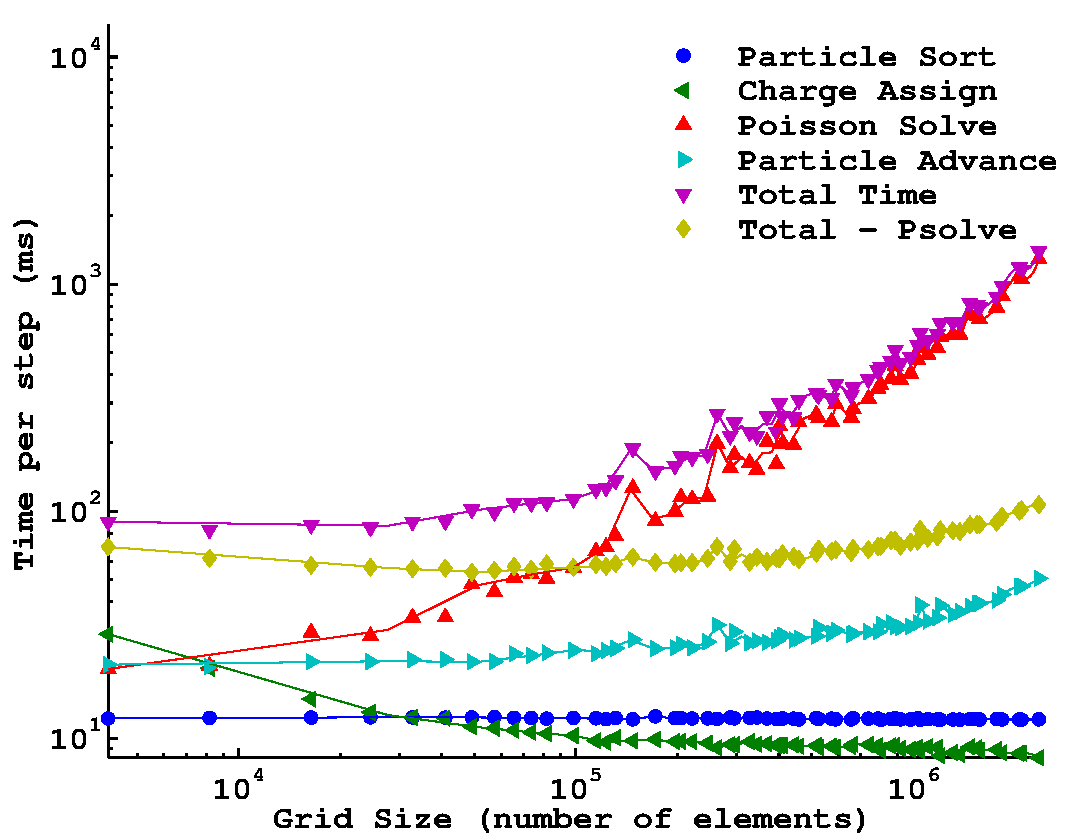
\includegraphics[width=6in]{performance/gridsize_scan8ptcls8bins.pdf}
%\end{center}
%\caption{Gridsize Scan with 8 million ptcls, and $8^3$ bins}
%\label{fig:grid_scan8ptcls8bins}
%\end{figure}


%\begin{figure}[H]
%\begin{center}
%
\includegraphics[width=6in]{performance/gridsize_scan8ptcls16bins.pdf}
%\end{center}
%\caption{Gridsize Scan with 8 million ptcls, and $16^3$ bins}
%\label{fig:grid_scan8ptcls16bins}
%\end{figure}


\begin{figure}
\begin{center}
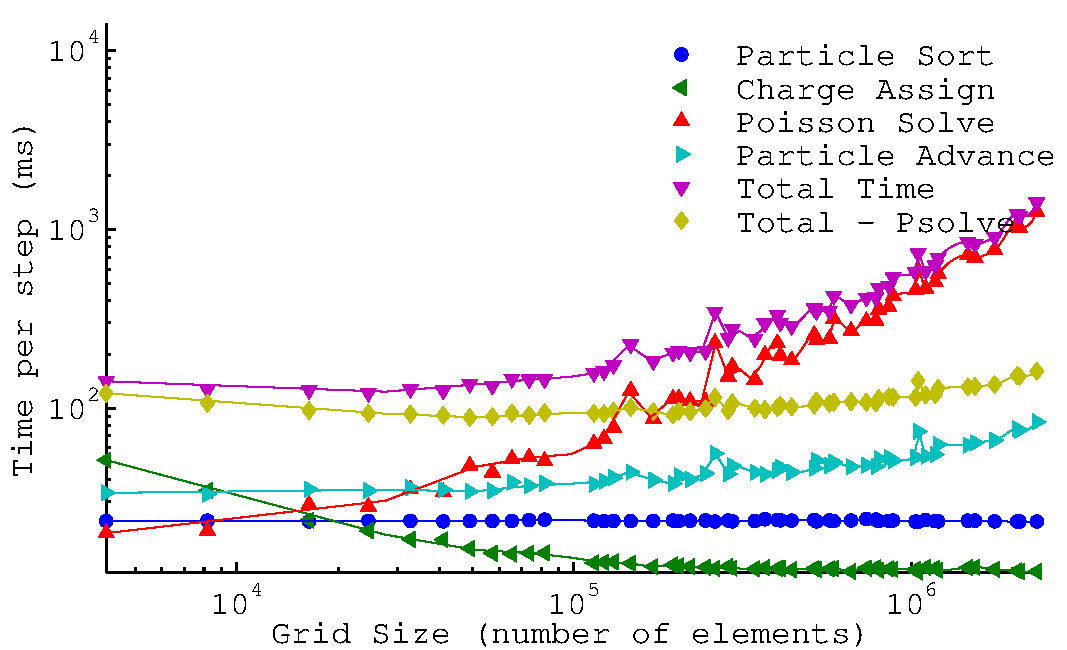
\includegraphics[width=6in]{performance/gridsize_scan16ptcls8bins.pdf}
\end{center}
\caption{Gridsize Scan with 16 million ptcls, and $8^3$ bins}
\label{fig:grid_scan16ptcls8bins}
\end{figure}

\begin{figure}
\begin{center}
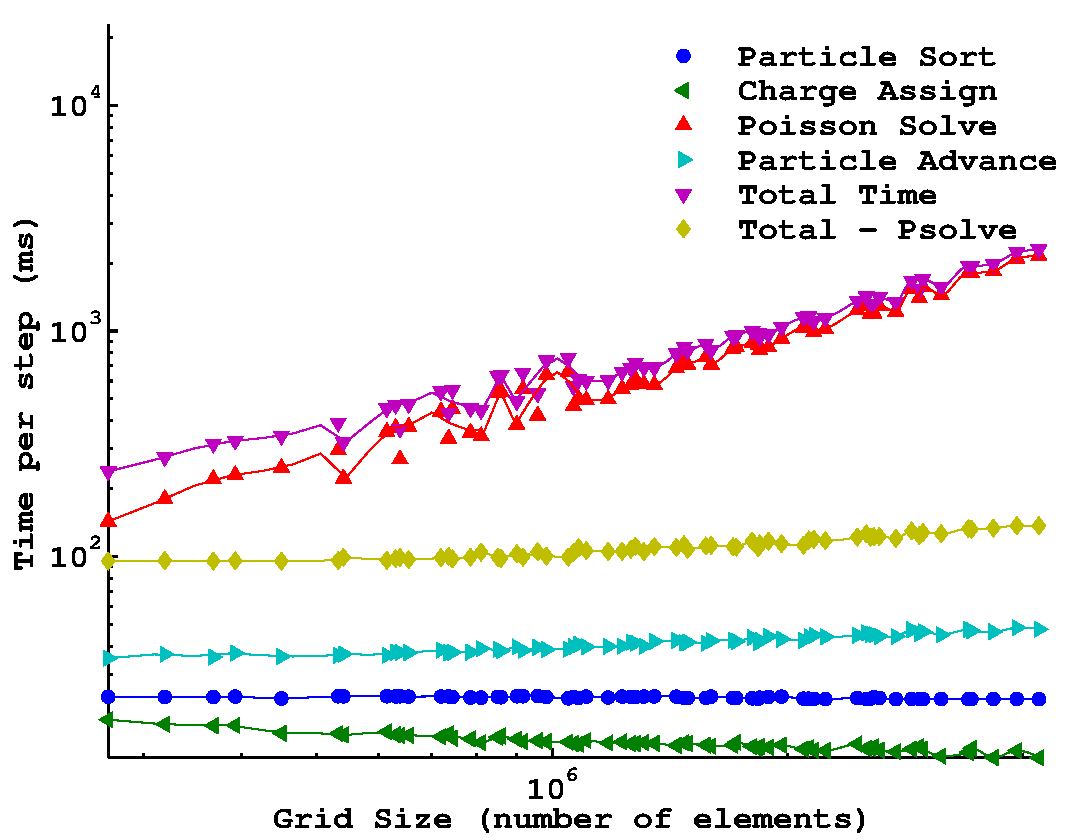
\includegraphics[width=6in]{performance/gridsize_scan16ptcls16bins.pdf}
\end{center}
\caption{Gridsize Scan with 16 million ptcls, and $16^3$ bins}
\label{fig:grid_scan16ptcls16bins}
\end{figure}

\begin{figure}
\begin{center}
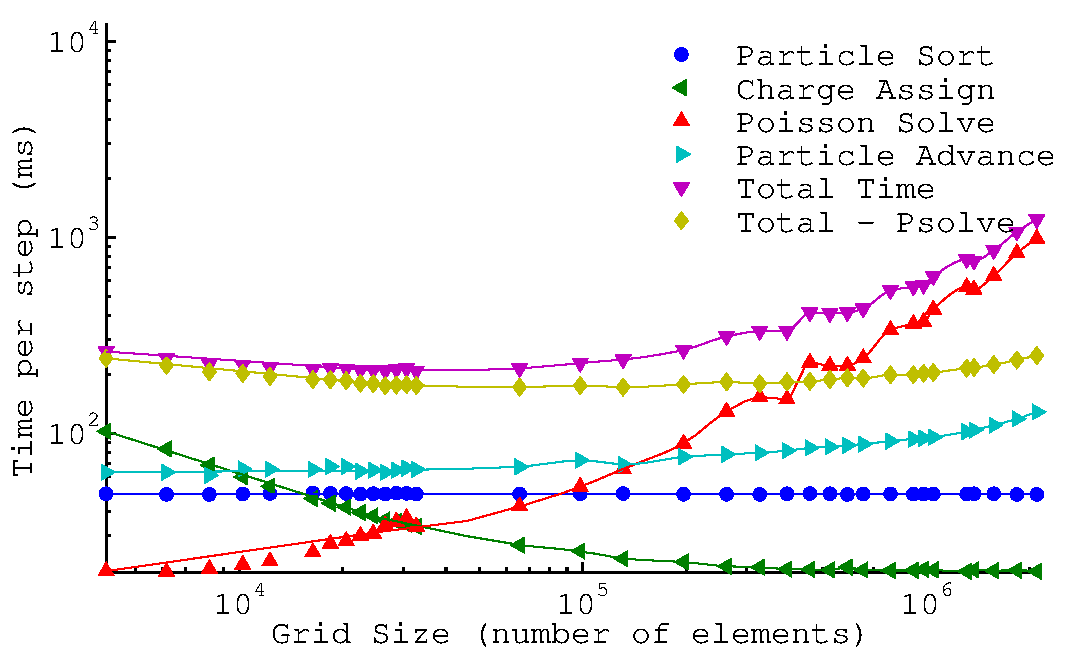
\includegraphics[width=6in]{performance/gridsize_scan34ptcls8bins.pdf}
\end{center}
\caption{Gridsize Scan with 34 million ptcls, and $8^3$ bins. Note how when the contribution from the poisson solve is removed there is a clear minimum at about $10^5$ elements. }
\label{fig:grid_scan34ptcls8bins}
\end{figure}

\begin{figure}
\begin{center}
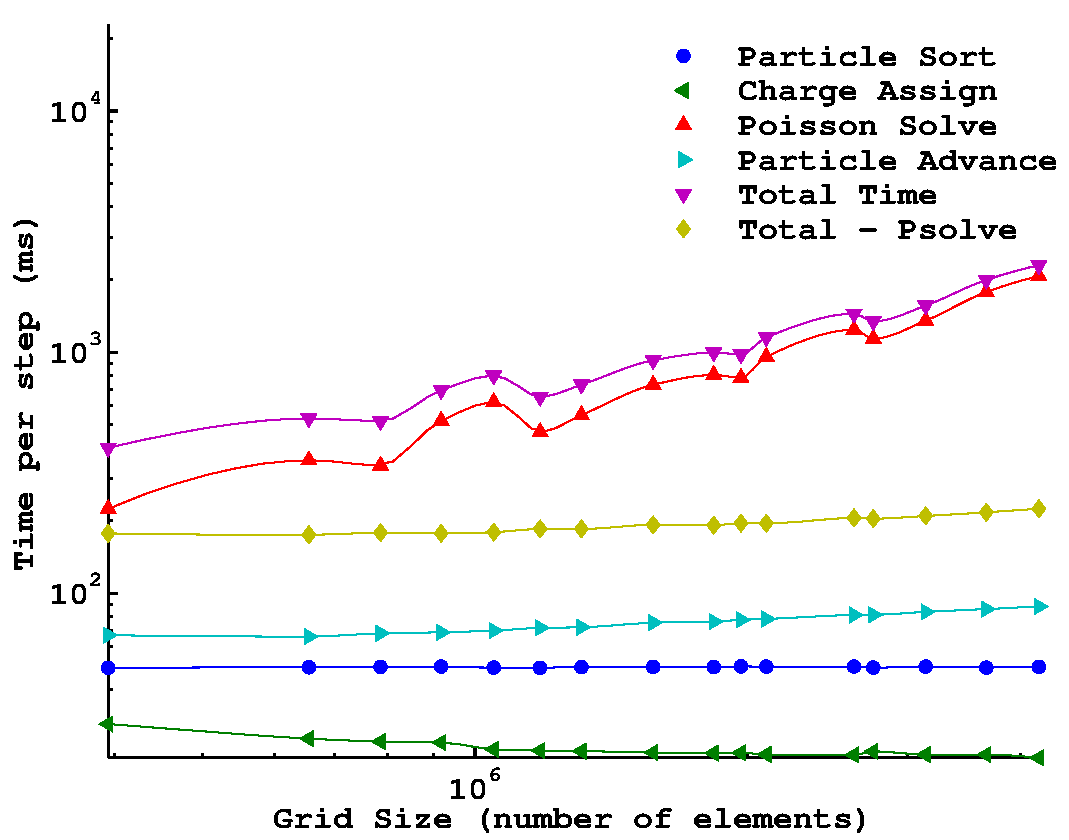
\includegraphics[width=6in]{performance/gridsize_scan34ptcls16bins.pdf}
\end{center}
\caption{Gridsize Scan with 34 million ptcls, and $16^3$ bins}
\label{fig:grid_scan34ptcls16bins}
\end{figure}

\begin{figure}
\begin{center}
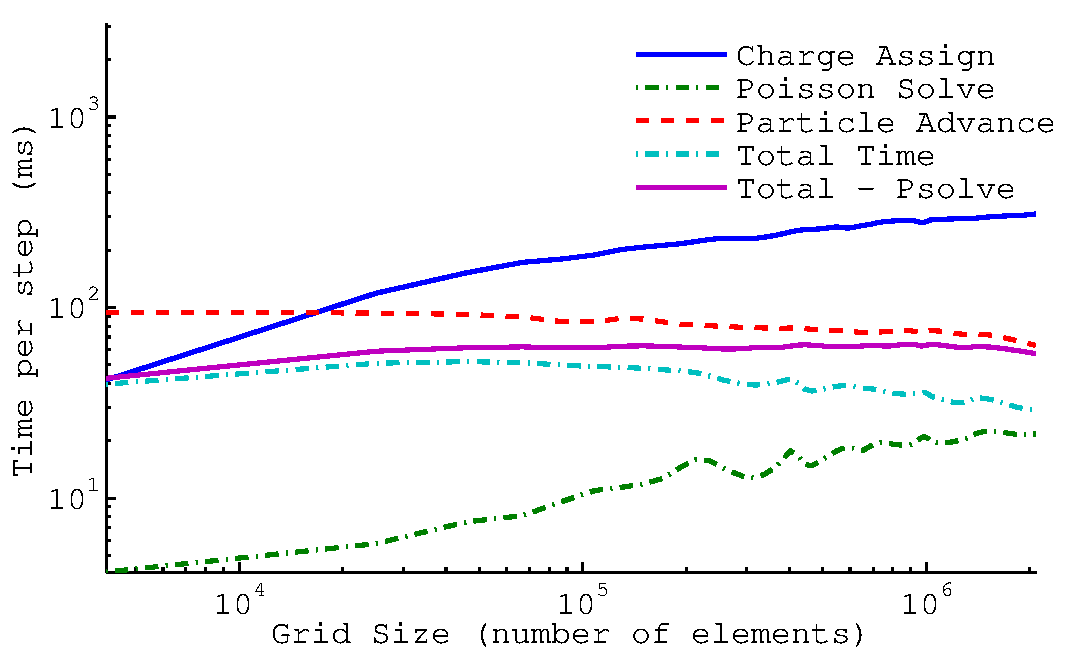
\includegraphics[width=6in]{performance/gridsize_speedup_scan.pdf}
\end{center}
\caption{Gridsize Speedup Scan with 34 million ptcls, and $8^3$ bins}
\label{fig:grid_scan34ptcls16bins}
\end{figure}

The more subtle scalings of the particle advance and charge assign can be seen in figures \ref{fig:grid_scan16ptcls8bins} through \ref{fig:grid_scan34ptcls16bins} in the cases where there are only $8^3$ bins, but do not continue their trends for $16^3$ bins. This behavior is due to the fact that these are not scalings with the absolute grid size, but rather scalings with sub-domain size.

Another point of interest is the scaling of the particle sort, note that it only scales with the number of particles and is completely independent of grid size. One might expect to find some small scaling based on the distance that particles have to be moved during the sort stage, or that with fewer sub-domains the radix sort would have fewer digits to process, but this is not the case. This means that some improvement can be made to the sort, namely using the number of bins as the upper limit on the bits for the radix sort to process. Hopefully this kind of feature will be available in future releases of the thrust library.



\subsection{Threadblock Sub-Domain Size}
In chapter 4 we discussed the scaling of both the particle advance and the charge assign subroutines with grid size. Smaller grids should lead to more atomic conflicts in the charge assign and thus longer run time. On the other hand, for the particle advance smaller grids mean that a larger fraction of the grid can be stored in cache, which leads to fewer global memory accesses. Taking these two effects together, we should see a clear minimum in the data. Figure \ref{fig:subdomain_size_scan} shows the time per step of each routine vs the size of the sub-domain. Correcting for the Poisson solve we do in fact see a minimum in the run time. 

\begin{figure}[H]
\begin{center}
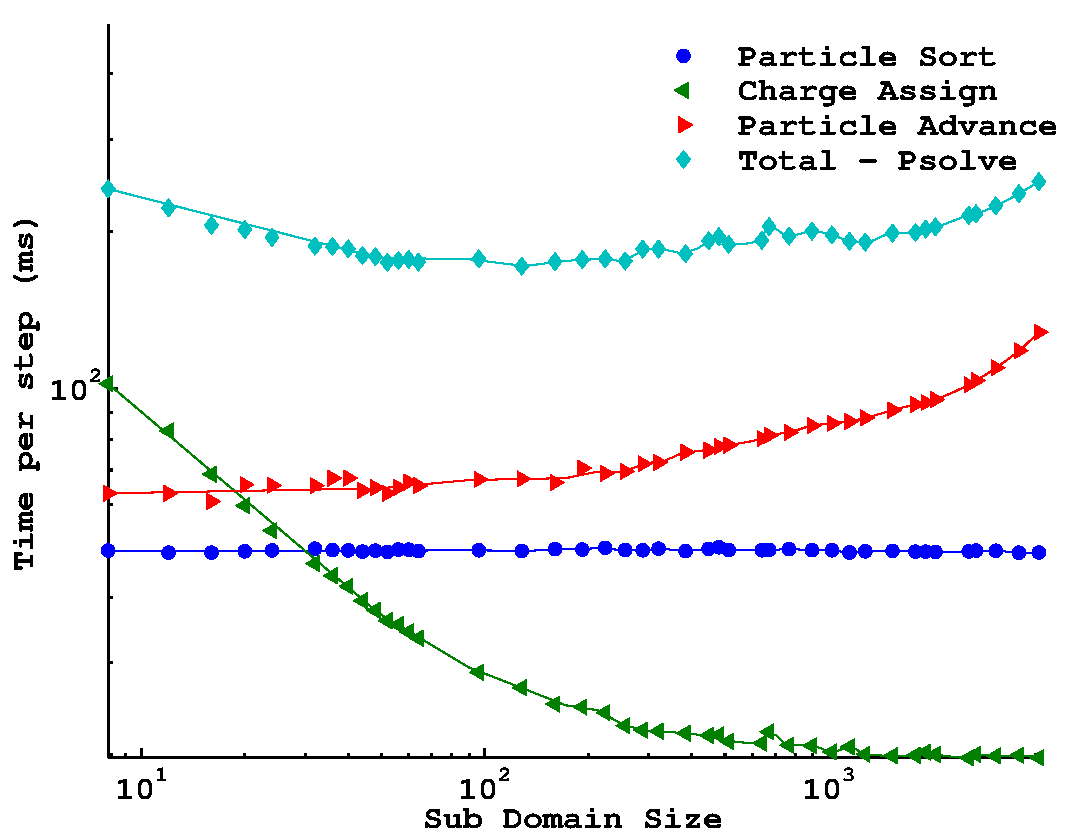
\includegraphics[width=6in]{performance/gridshape_scan.pdf}
\end{center}
\caption{Sub Domain Size scan, also known as bin size, for 34 million particles. Note the minimum in the total - psolve run time.}
\label{fig:subdomain_size_scan}
\end{figure}


	\section{Kernel Parameters Scan}
One important performance consideration for GPU computing is ensuring that every thread performs enough work to warrant the cost of its creation. For the case of the advancing kernel we adjusted the number of particles processed by each thread. This is essentially a parameter that could be optimized with through auto-tuning, and will likely vary based on the hardware configuration. We performed such a scan with the advancing kernel, ranging the number of particles processed per thread from 3 to 16. The results of this scan can can be seen in figure \ref{fig:kernel_param_scan}.

\begin{figure}[H]
\begin{center}
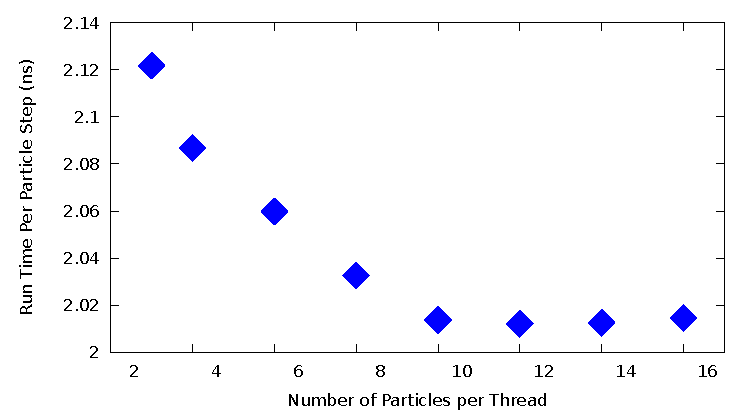
\includegraphics[width=6in]{performance/kernel_param.pdf}
\end{center}
\caption{Adjusting the amount of work per thread for the advancing kernel.}
\label{fig:kernel_param_scan}
\end{figure}

As we can see from the figure, there is a minimum around 10 particles per thread, which is about 5\% faster than the 3 particles per thread case. Now a 5\% increase may not seem like much in the context of the GPU advancing kernel, but we have to take it in context with the speedup that we have already achieved. If we recognize that the GPU advancing routine is 80 times faster than the CPU version, then a 5\% performance boost brings the GPU version to 84 times faster than the CPU version. 

%%%%%%%%%%%%%%%%%%%%%%%%%%%%%%%%%%%%
	\section{Texture Performance}
%%%%%%%%%%%%%%%%%%%%%%%%%%%%%%%%%%%%

One of the more interesting concepts that we investigated was the use of textures as a storage structure for both the potential, and the Poisson solve sparse matrix diagonals. Several comparisons between the two can be seen in figures \ref{fig:texture_tests64} and \ref{fig:texture_tests128}. These tests were performed using 42 million particles with 200 time steps on $128^3$ and $64^3$ grids. We also varied the number of cells per sorting bin (cpb) in order to determine how the performance gain from using texture memory varies with how many possible mesh points an execution block of particles can access.

\begin{figure}
\begin{center}
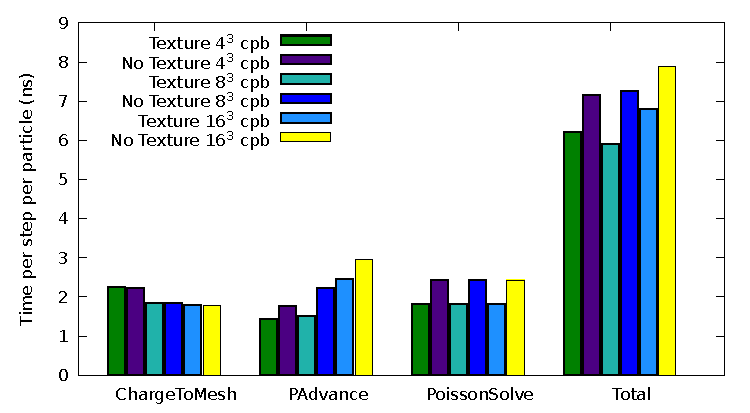
\includegraphics[width=6in]{performance/texture_tests64.pdf}
\end{center}
\caption{Comparison between texture enabled kernels at various bin sizes. Tests used 42 million particles with 200 time steps on a $64^3$ grid.}
\label{fig:texture_tests64}
\end{figure}

\begin{figure}
\begin{center}
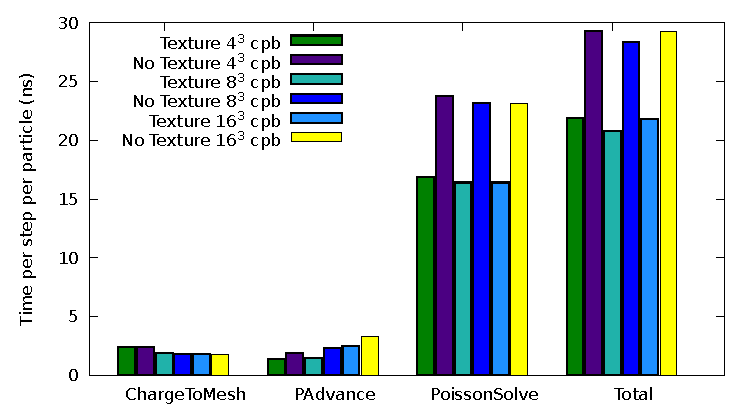
\includegraphics[width=6in]{performance/texture_tests128.pdf}
\end{center}
\caption{Comparison between texture enabled kernels at various bin sizes. Tests used 42 million particles with 200 time steps on a $128^3$ grid.}
\label{fig:texture_tests128}
\end{figure}

As you can see from figures \ref{fig:texture_tests64} and \ref{fig:texture_tests128}, utilizing texture memory does provide a noticeable performance boost for the Poisson solve, and a small boost for the particle advance. Additionally, it is interesting to not that for particle advancing varying the number of cells per bin from $4^3$ to $8^3$ does not change the run time of the texture run. The particle advance without textures becomes slower as the number of cells per bin increases, but there is a threshold for the texture based routine.

It is likely that more data structures could be changed to textures, or surfaces for read/write data structures. The Poisson solve in particular could benefit from additional texture/surface memory usage. The primary barrier to this is not performance, but implementation difficulty. Textures are not easy to incorporate into code due to the fact that they cannot be passed as function arguments, and must be declared within the same file scope as they are used. Another downside to textures is the process of ``binding" global memory to the texture reference, which can be expensive.  


